\documentclass[12pt]{article}
\usepackage{polski}
\usepackage[utf8]{inputenc}
\usepackage{amsfonts}
\usepackage{amsmath}
\usepackage{enumitem}
\usepackage{graphicx}
\usepackage{float}
\usepackage{centernot}
\setlength{\parskip}{1em}


\begin{document}
	\title{Sprawozdanie\\Metody Numeryczne 2, laboratorium 3}
	\author{Grzegorz Rozdzialik (D4, grupa lab. 2)}
	\maketitle	
	
	\section{Zadanie}
	{\Large Temat \textbf{3}, zadanie \textbf{33}:}\\
	Obliczanie całek\
	$$\iint_D f(x, y) \,dx\,dy$$
	na obszarze
	$$D = \{(x, y) \in \mathbb{R}^2: |x| + |y| \leq 1\}$$
	przez podział $D$ na $4n^2$ trójkątów przystających i zastosowanie na każdym z nich kwadratury rzędu 4-go.
	
	Obszar $D$ został przedstawiony na rysunku nr \ref{D-area}, jest to romb o środku $P_0 = (0, 0)$ i wierzchołkach
	\begin{align*}
		P_1 & = (1, 0)  \\
		P_2 & = (0, 1)  \\
		P_3 & = (-1, 0) \\
		P_4 & = (0, -1)
	\end{align*}
	
	\begin{figure}[H]
		\centering
		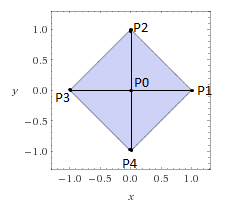
\includegraphics[scale=1.5]{images/D-area.png}
		\caption{Obszar $D$}
		\label{D-area}
	\end{figure}

	
	\section{Opis metody}
	\subsection{Podział rombu na $4n^2$ trójkątów}
	W celu podzielenia obszaru $D$ na $4n^2$ trójkątów użyto podział na 4 ćwiartki $D_1, D_2, D_3, D_4$ na podstawie osi układu współrzędnych. Podział ten został przedstawiony na rysunku nr \ref{D-quarters}.
	
	\begin{figure}[H]
		\centering
		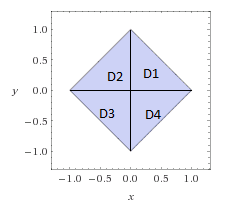
\includegraphics[scale=1.5]{images/D-quarters.png}
		\caption{Podział $D$ na ćwiartki}
		\label{D-quarters}
	\end{figure}

	Następnie każdą z ćwiartek podzielono na $n^2$ trójkątów według następującej reguły:
	\begin{enumerate}
		\item Każdy bok podzielono na $n$ równych części (punkty podziału nazwijmy węzłami).
		\item Węzły leżące na dwóch różnych bokach trójkąta i równoodległe od trzeciego z boków łączymy prostymi. Proste te będą wtedy równoległe do jednego z boków.
	\end{enumerate}

	Przykładowy schemat podziału ćwiartki $D_1$ z $n = 3$ ($D_1$ podzielono na 9 trójkątów przystających) został umieszczony na rysunku nr \ref{triangle-division}.
	
	\begin{figure}[H]
		\centering
		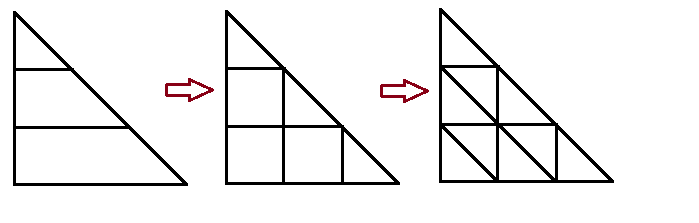
\includegraphics[]{images/triangle-division.png}
		\caption{Podział $D_1$ na 9 (= $3^2$) trójkątów}
		\label{triangle-division}
	\end{figure}

	Wszystkie $n^2$ trójkątów po podziale mają takie samo pole, równe $p = \frac{P}{n^2}$, gdzie $P = |D_1| = |D_2| = |D_3| = |D_4|$.
	
	Na każdym z tych trójkątów obliczamy wartość kwadratury 4-go rzędu:
	\begin{align}
		S(f) = & \frac{p}{60} \Bigg[  27f(P_{012}) + 3 \Big( f(P_{01}) + f(P_{02}) + f(P_{12}) \Big)  \nonumber \\
		       & + 8\Big( f(P_0) + f(P_1) + f(P_2) \Big) \Bigg] \label{kwadratura}
	\end{align}
	
	gdzie $f$ jest zadaną funkcją podcałkową, $p$ zdefiniowane jak poprzednio, $P_0, P_1, P_2$ są wierzchołkami trójkąta po podziale, $P_{i,j} = \frac{P_i + P_j}{2}$ są środkami boków trójkąta, $P_{012} = \frac{P_0 + P_1 + P_2}{3}$ jest środkiem ciężkości trójkąta.
	
	
	\subsection{Wyznaczanie współrzędnych wierzchołków trójkątów po podziale}
	Aby zastosować kwadraturę \eqref{kwadratura} należy znać współrzędne wierzchołków. Zauważmy, że trójkąty po podziale można pogrupować w wiersze tak, że w pierwszym wierszu znajduje się jeden trójkąt, a w każdym kolejnym są o 2 więcej. Ostatni wiersz ($n$-ty) posiada $2n - 1$ trójkątów.
	
	W $i$-tym wierszu jest $2i - 1$ trójkątów. Podział $i$-tego wiersza wraz z numerami kolejnych trójkątów został pokazany na rysunku nr \ref{division-row}.
	
	\begin{figure}[H]
		\centering
		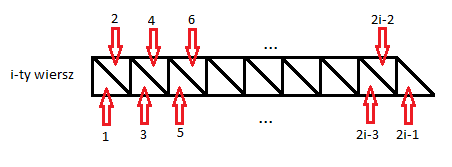
\includegraphics[]{images/division-row.png}
		\caption{Podział $i$-tego wiersza}
		\label{division-row}
	\end{figure}

	Niech $P_0, P_1, P_2$ będą współrzędnymi wierzchołków trójkąta przed podziałem zdefiniowanym analogicznie jak na rysunku \ref{D-area}. Podział na wiersze rozpoczynamy od $P_2$, zatem trójkąt po podziale, którego jednym z wierzchołków będzie $P_2$ znajdzie się w pierwszym wierszu.
	
	Zdefiniujmy następujące zmienne:
	\begin{align*}
		h_x & = \frac{P_1 - P_0}{n} \\
		h_y & = \frac{P_0 - P_2}{n}
	\end{align*}
	Wtedy $h_x$ będzie wektorem, o jaki należy się przesunąć, aby uzyskać współrzędne kolejnej kolumny, natomiast $h_y$ będzie wektorem, o jaki należy się przesunąć, aby uzyskać współrzędne kolejnego wiersza. Zakładam, że każda kolumna oprócz ostatniej w danym wierszu posiada 2 trójkąty.
	
	Zatem jeżeli trójkąt ma nieparzysty indeks, to znajduje się bliżej kolejnego wiersza ("na dole"), a te z indeksem parzystym są bliżej poprzedniego wiersza ("na górze"), jak na rysunku \ref{division-row}.
	
	Aby wyznaczyć współrzędne trójkąta o indeksach $(i, j)$, gdzie $i \in \{1, 2, \dots, n\}$, $j \in \{1, 2, \dots, 2i-1\}$, w oparciu o współrzędne wierzchołka $P_2$ należy rozważyć dwa przypadki:
	
	\begin{enumerate}[label=\textbf{\Roman*}]
		\item $2 \mid j$
		
		\begin{figure}[H]
			\centering
			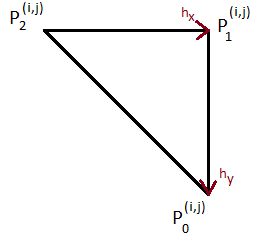
\includegraphics[]{images/triangle-j-even.png}
			\caption{Trójkąt po podziale, gdy $j$ - parzyste}
			\label{triangle-j-even}
		\end{figure}
		
		Wtedy
		\begin{align*}
			P_2^{(i,j)} & = P_2 + (i-1)h_y + \frac{j-2}{2}h_x \\
			P_0^{(i,j)} & = P_2^{(i,j)} + h_y                   \\
			P_1^{(i,j)} & = P_2^{(i,j)} + h_x
		\end{align*}
		
		
		\pagebreak
		
		\item $2 \centernot\mid j$
		
		\begin{figure}[H]
			\centering
			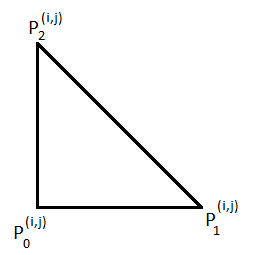
\includegraphics[]{images/triangle-j-odd.png}
			\caption{Trójkąt po podziale, gdy $j$ - nieparzyste}
			\label{triangle-j-odd}
		\end{figure}
		
		Wtedy
		\begin{align*}
		P_2^{(i,j)} & = P_2 + (i-1)h_y + \frac{j-1}{2}h_x \\
		P_0^{(i,j)} & = P_2^{(i,j)} + h_y                   \\
		P_1^{(i,j)} & = P_0^{(i,j)} + h_x
		\end{align*}
	\end{enumerate}
	gdzie $P_k^{(i,j)}$ oznacza współrzędne k-tego wierzchołka trójkąta o indeksach $(i, j)$ po podziale (analogicznie do rysunków w podpunktach).
	
	
	
	
	
	\section{Implementacja metody}
	Metoda zaimplementowana jest na podstawie czterech funkcji oraz jednego skryptu pozwalającego na łatwe jej wykorzystanie i porównanie z funkcją \textit{integral2} z MATLABa:
	\begin{itemize}
		\item $[h_x, h_y, P] = computeDivisionProperties(P_0, P_1, P_2, n)$
		
		Funkcja oblicza własności podziału trójkąta o wierzchołkach $P_0, P_1, P_2$ na $n^2$ trójkątów przystających (zgodnie z powyższym opisem metody). Zwraca wektory $h_x, h_y$ oraz pole trójkąta $P$ po podziale.
		
		
		\item $[P_0^{(i,j)}, P_1^{(i,j)}, P_2{(i,j)}] = computeSingleTriangleCoordinates(P_2, h_x, h_y, i, j)$
		
		Funkcja oblicza współrzędne trójkąta o indeksie $(i, j)$ po podziale na podstawie współrzędnej $P_2$ trójkąta przed podziałem oraz wektorów $h_x, h_j$.
		
		
		\item $S = integrateSingleTriangle(f, P_0, P_1, P_2, P)$
		
		Funkcja przybliża wartość całki z funkcji podcałkowej $f$ na trójkącie o polu $P$ i wierzchołkach $P_0, P_1, P_2$, używając do tego kwadratury \eqref{kwadratura}.
		
		
		\item $S = numericalInterpolationTriangle(f, P_0, P_1, P_2, n)$
		
		Funkcja przybliża wartość całki z funkcji podcałkowej $f$ na trójkącie o wierzchołkach $P_0, P_1, P_2$, dzieląc go na $n^2$ trójkątów przystających.
		
		Funkcja używa $computeDivisionProperties$ do uzyskania własności podziału ($h_x, h_y, P$), a następnie wykonuje przybliżenie całki na każdym z trójkątów po podziale używając funkcji $computeSingleTriangleCoordinates$ do uzyskania współrzędnych tego trójkąta, oraz $integrateSingleTriangle$ do uzyskania wartości kwadratury.
		
		\item $integrateDiamond$
		
		Skrypt pozwalający określić funkcję podcałkową $f$ oraz parametr $n$ określający liczbę podziałów. Wykonuje zadanie - przybliża całkę na obszarze $D$ (rysunek \ref{D-area}).
		
		Skrypt dodatkowo podaje informacje o szybkości działania metody oraz porównuje ją z funkcją $integral2$ dostępną w MATLABie.
	\end{itemize}

	Funkcji można używać do przybliżania całki na dowolnym trójkącie, zatem nie musi być to romb podzielony na 4 trójkąty. Wystarczy zmodyfikować skrypt $integrateDiamond$.
	
	Nie jest to jednak tematem zadania, więc postanowiono zostawić to jako zadanie dla ciekawego czytelnika.
	
	
	
	
	\section{Poprawność metody}
	TODO
	
	
	
	
	
	
	\section{Przykłady}
	\begin{enumerate}[label=\textbf{Przykład \arabic*}]
		\item
		TODO
		
	\end{enumerate}
	
	
	
	
	
	
	\section{Wnioski}
	\begin{enumerate}
		\item TODO
	\end{enumerate}

	
	
	
	
	
	\section{Funkcja do testowania}
	TODO
	
	
	
	
	
	\section{Bibliografia}
	\begin{enumerate}
		\item Informacje z wykładu \textit{Metod numerycznych 2} (wydział MiNI PW, dr Iwona Wróbel) (w szczególności wzór na kwadraturę rzędu 4 na trójkącie)
	\end{enumerate}
	
\end{document}